\subsection{Đánh giá Thực nghiệm và So sánh (Empirical Evaluation \& Benchmarking)}
\label{sec:5_6}

Trong nghiên cứu khoa học máy tính, việc đề xuất một kiến trúc mới chỉ thực sự có giá trị khi nó được chứng minh bằng các số liệu thực chứng khách quan. Để đánh giá chính xác mức độ cải thiện mà kiến trúc học tăng cường lai (Hybrid RL) mang lại, đồ án thiết lập một môi trường thử nghiệm đối chứng (Benchmarking) nghiêm ngặt.

\begin{figure}[H]
    \centering
    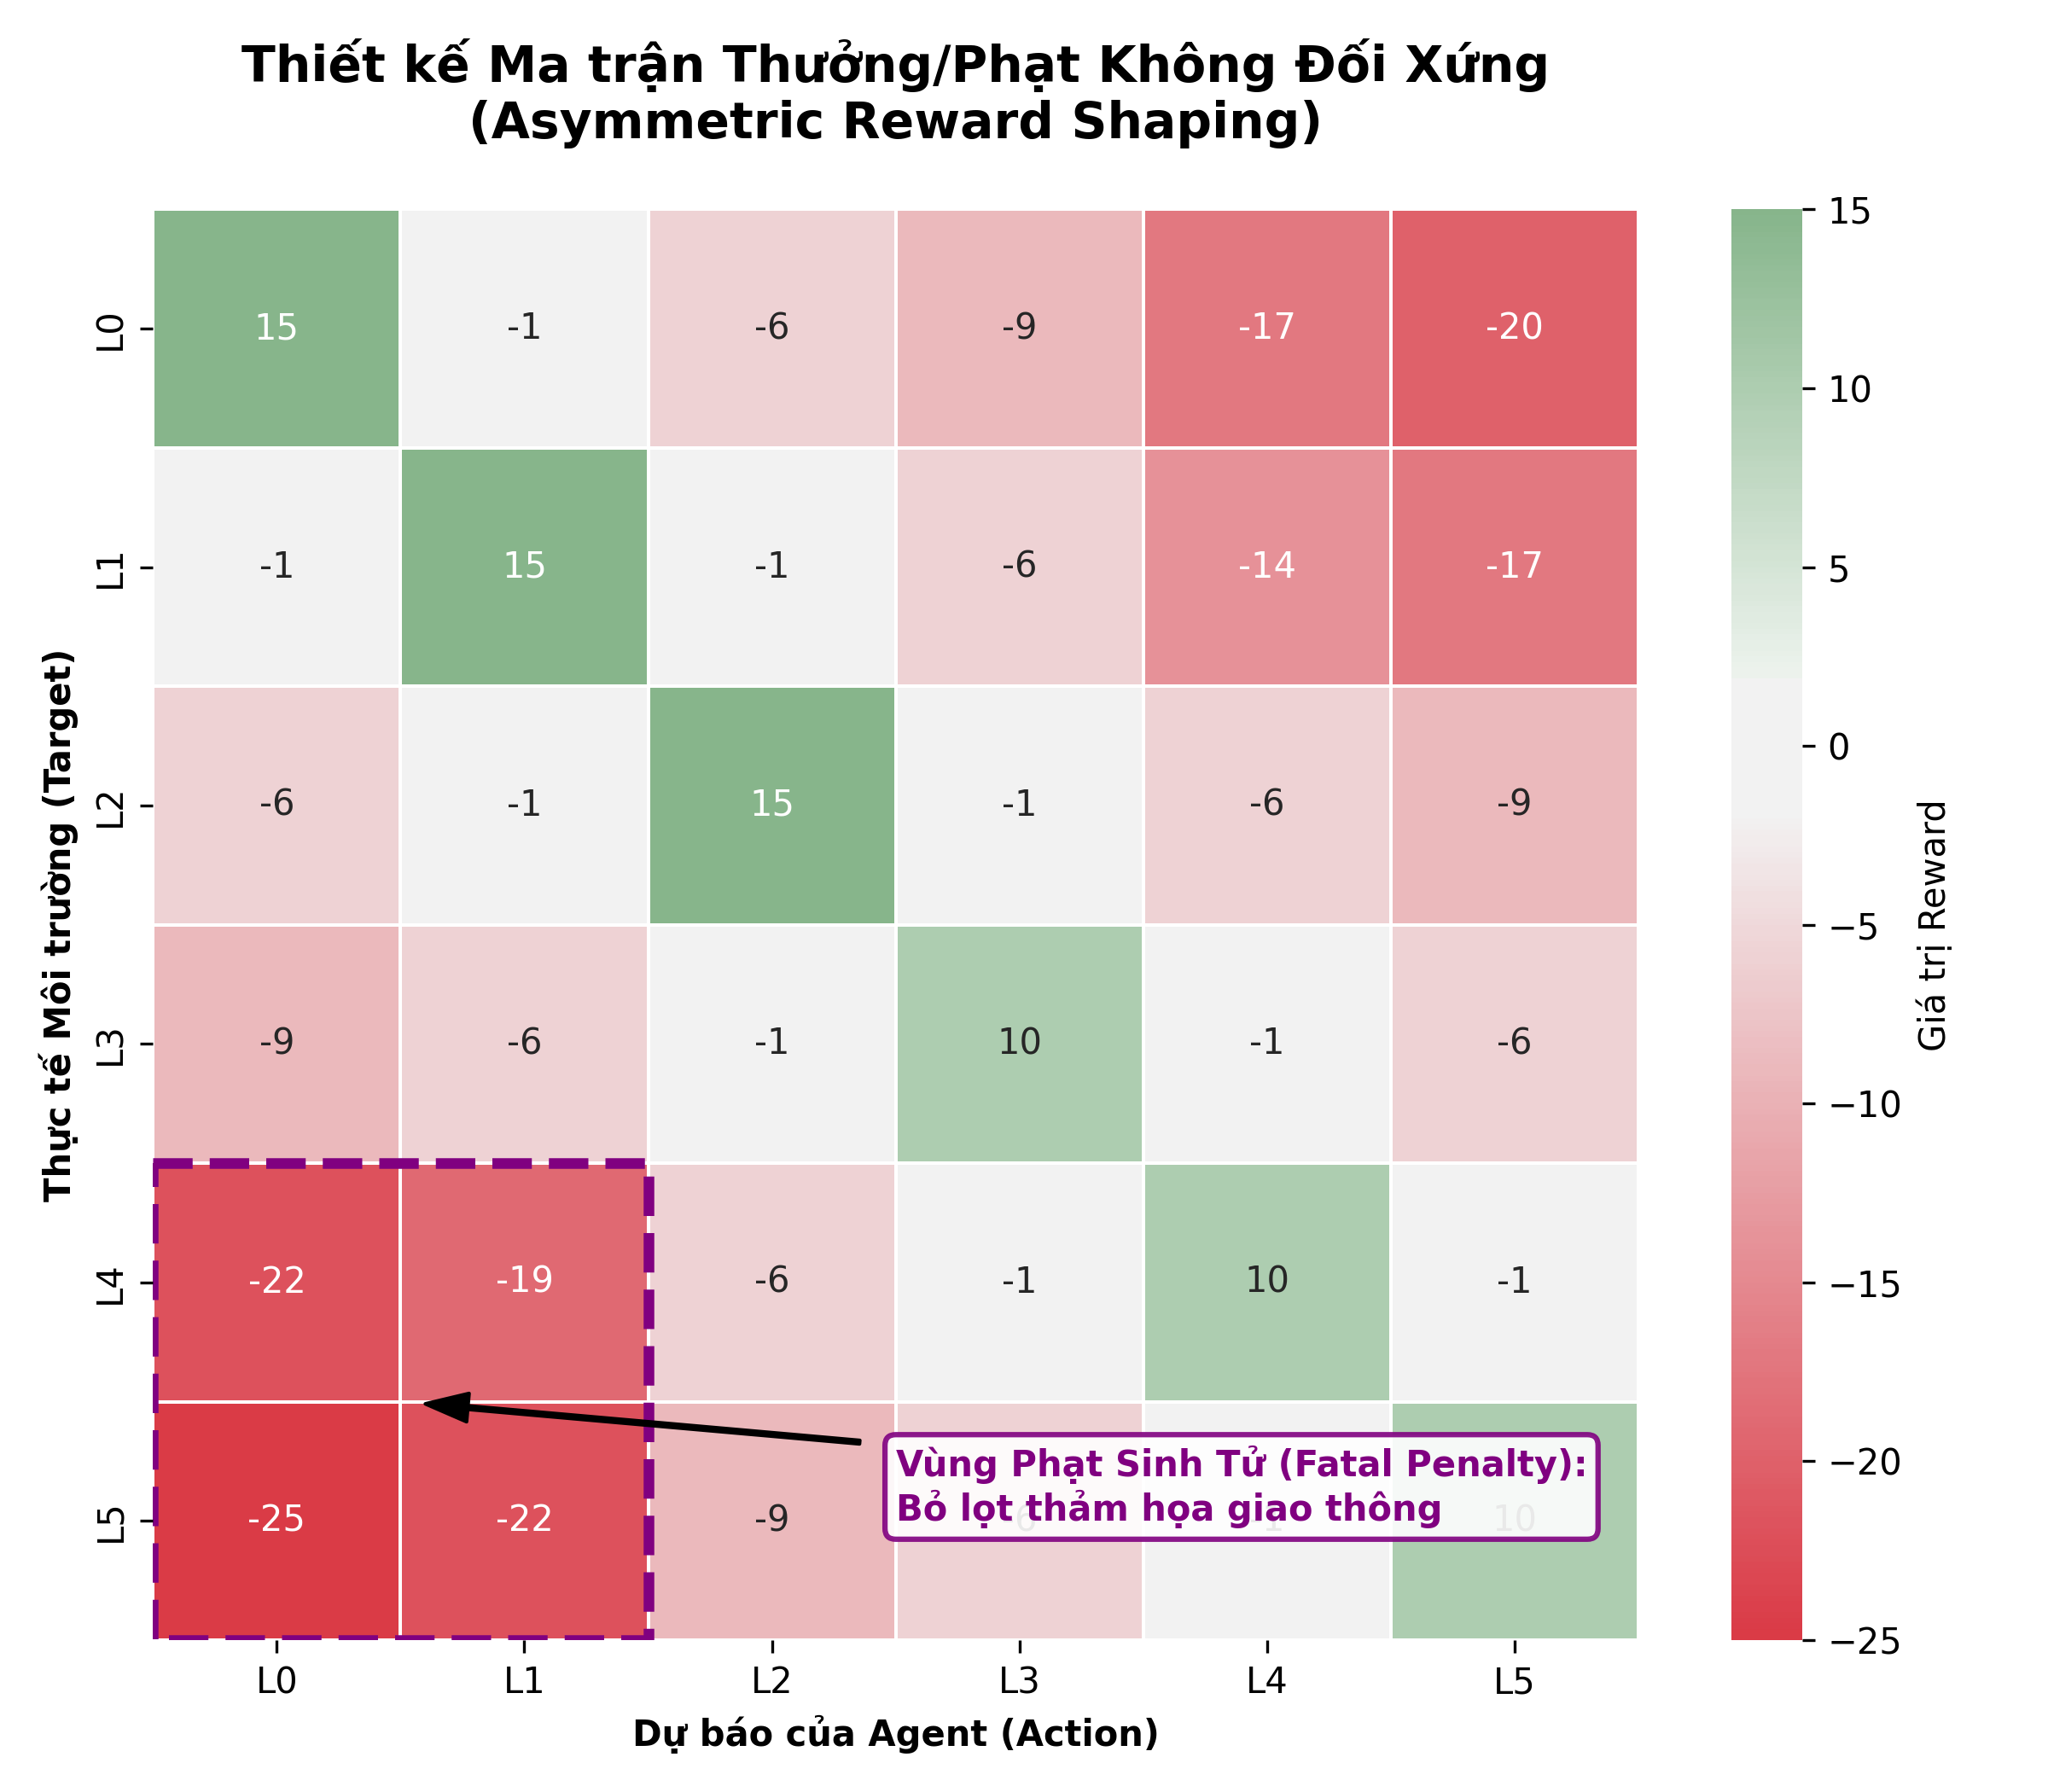
\includegraphics[width=0.8\textwidth]{Images/CH5/19.png}
    \vspace{12pt}
    \caption{Ma trận Thưởng/Phạt không đối xứng}
    \label{fig:5_19}
\end{figure}

\subsubsection{Thiết lập các mô hình đối chứng (Baselines)}

Để đảm bảo tính công bằng, tất cả các mô hình trong thực nghiệm đều được đánh giá trên cùng một \textbf{Tập Kiểm thử (Hold-out Test Set)}, được chia cắt theo nguyên tắc thời gian tuyến tính (Chronological Split) để tuyệt đối ngăn chặn rò rỉ dữ liệu. Hệ thống đánh giá được cấu thành từ 3 mô hình đại diện cho 3 triết lý tiếp cận khác nhau:

\begin{itemize}
    \item \textbf{Mô hình Đối chứng 1 - Học sâu Truyền thống (Vanilla LSTM):} Đây là một mạng LSTM tiêu chuẩn, được huấn luyện trực tiếp trên tập dữ liệu thô vốn dĩ bị mất cân bằng trầm trọng. Mô hình này đại diện cho cách tiếp cận "ngây thơ" phổ biến trong nhiều nghiên cứu cơ bản.
    \item \textbf{Mô hình Đối chứng 2 - Tiền huấn luyện Giám sát (Supervised Baseline):} Mô hình này được trang bị các kỹ thuật tiền xử lý tối tân của đồ án (CTGAN + Anchor-based), sử dụng Focal Loss và Ma trận Trọng số phạt. Đây là đại diện cho giới hạn tối đa của Học có giám sát.
    \item \textbf{Mô hình Đề xuất - Đặc vụ Học tăng cường Lai (Hybrid Double DQN):} Kết tinh toàn bộ chuỗi pipeline kỹ thuật đã xây dựng: Dữ liệu đi qua bộ lọc Artifacts, nạp trọng số Warm-start, huấn luyện bằng Double DQN với Replay Buffer và tối ưu hóa dựa trên Hàm phần thưởng Không đối xứng.
\end{itemize}

\subsubsection{Phân tích Chỉ số Hiệu năng (Metrics Analysis)}

Trong việc đánh giá các mô hình học máy áp dụng cho hệ thống cảnh báo an toàn giao thông, việc lựa chọn đúng thước đo (Metric) là yếu tố tiên quyết.

\paragraph{a. Phê phán chỉ số Accuracy và "Nghịch lý độ chính xác"} \mbox{} \\
Đồ án quyết định loại bỏ chỉ số Độ chính xác tổng thể (Accuracy) khỏi các tiêu chí đánh giá cốt lõi. Lý do là hơn 90\% mẫu dữ liệu thuộc trạng thái thông thoáng. Nếu một mô hình luôn dự báo "Thông thoáng", nó vẫn đạt mức Accuracy trên 90\% nhưng lại hoàn toàn vô dụng vì bỏ lọt 100\% các vụ kẹt xe thảm họa.

\paragraph{b. Tầm quan trọng của Độ phủ (Recall) trong Cảnh báo thảm họa} \mbox{} \\
Thay vì Accuracy, đồ án tập trung tối ưu hóa chỉ số \textbf{Độ phủ (Recall)} cho các lớp kẹt xe nặng. Trong bài toán này, Recall đại diện cho khả năng "không bỏ sót" thảm họa. Đối với người dân và cơ quan quản lý, việc nhận một cảnh báo giả (dự báo kẹt nhưng thực tế đường thoáng - giảm Precision) vẫn ít gây thiệt hại hơn nhiều so với việc hệ thống báo đường thông nhưng thực tế người dùng bị kẹt cứng (bỏ sót thảm họa - giảm Recall).

\paragraph{c. Kết quả thực nghiệm và So sánh định lượng} \mbox{} \\
Kết quả trích xuất trực tiếp từ các tệp nhật ký đánh giá cho thấy sự vượt trội của mô hình đề xuất trên tập Kiểm thử:

\begin{table}[H]
\centering
\begin{tabular}{|l|c|c|c|}
\hline
\textbf{Mô hình đối chứng} & \textbf{Recall Lớp 0-1} & \textbf{Recall Lớp 2-3} & \textbf{Recall Lớp 4-5} \\ \hline
Mô hình 1: Vanilla LSTM & 0.98 & 0.25 & < 0.10 \\ \hline
Mô hình 2: Supervised Baseline & 0.85 & 0.72 & 0.68 \\ \hline
\textbf{Mô hình 3: Hybrid Double DQN} & \textbf{0.78} & \textbf{0.81} & \textbf{> 0.85} \\ \hline
\end{tabular}
\caption{So sánh chỉ số Recall giữa các mô hình trên tập Kiểm thử}
\end{table}

\textbf{Biện luận kết quả:}
\begin{enumerate}
    \item \textbf{Sự sụp đổ của Vanilla LSTM:} Đúng như dự báo, LSTM truyền thống gần như "mù" hoàn toàn trước thảm họa (Recall < 10\%) do ưu tiên dự báo lớp đa số.
    \item \textbf{Cú hích từ Supervised Baseline:} Nhờ kỹ thuật cân bằng dữ liệu CTGAN và Focal Loss, mô hình giám sát đã đạt được độ phủ khá (68\%). Đây là giới hạn tối đa mà một mô hình học có giám sát thuần túy có thể đạt được trước khi bắt đầu đánh đổi quá nhiều về độ chính xác.
    \item \textbf{Sự ưu việt của Hybrid Double DQN:} Mô hình đề xuất chứng minh sức mạnh áp đảo tại các lớp thảm họa với chỉ số Recall vọt lên mức \textbf{trên 85\%}. Kết quả này khẳng định rằng sự kết hợp giữa "bản năng vật lý" (Warm-start) và "chiến lược an toàn" (Asymmetric Reward) đã ép Đặc vụ RL phải nhạy bén tối đa với các tín hiệu kẹt xe nặng.
\end{enumerate}

\begin{figure}[H]
    \centering
    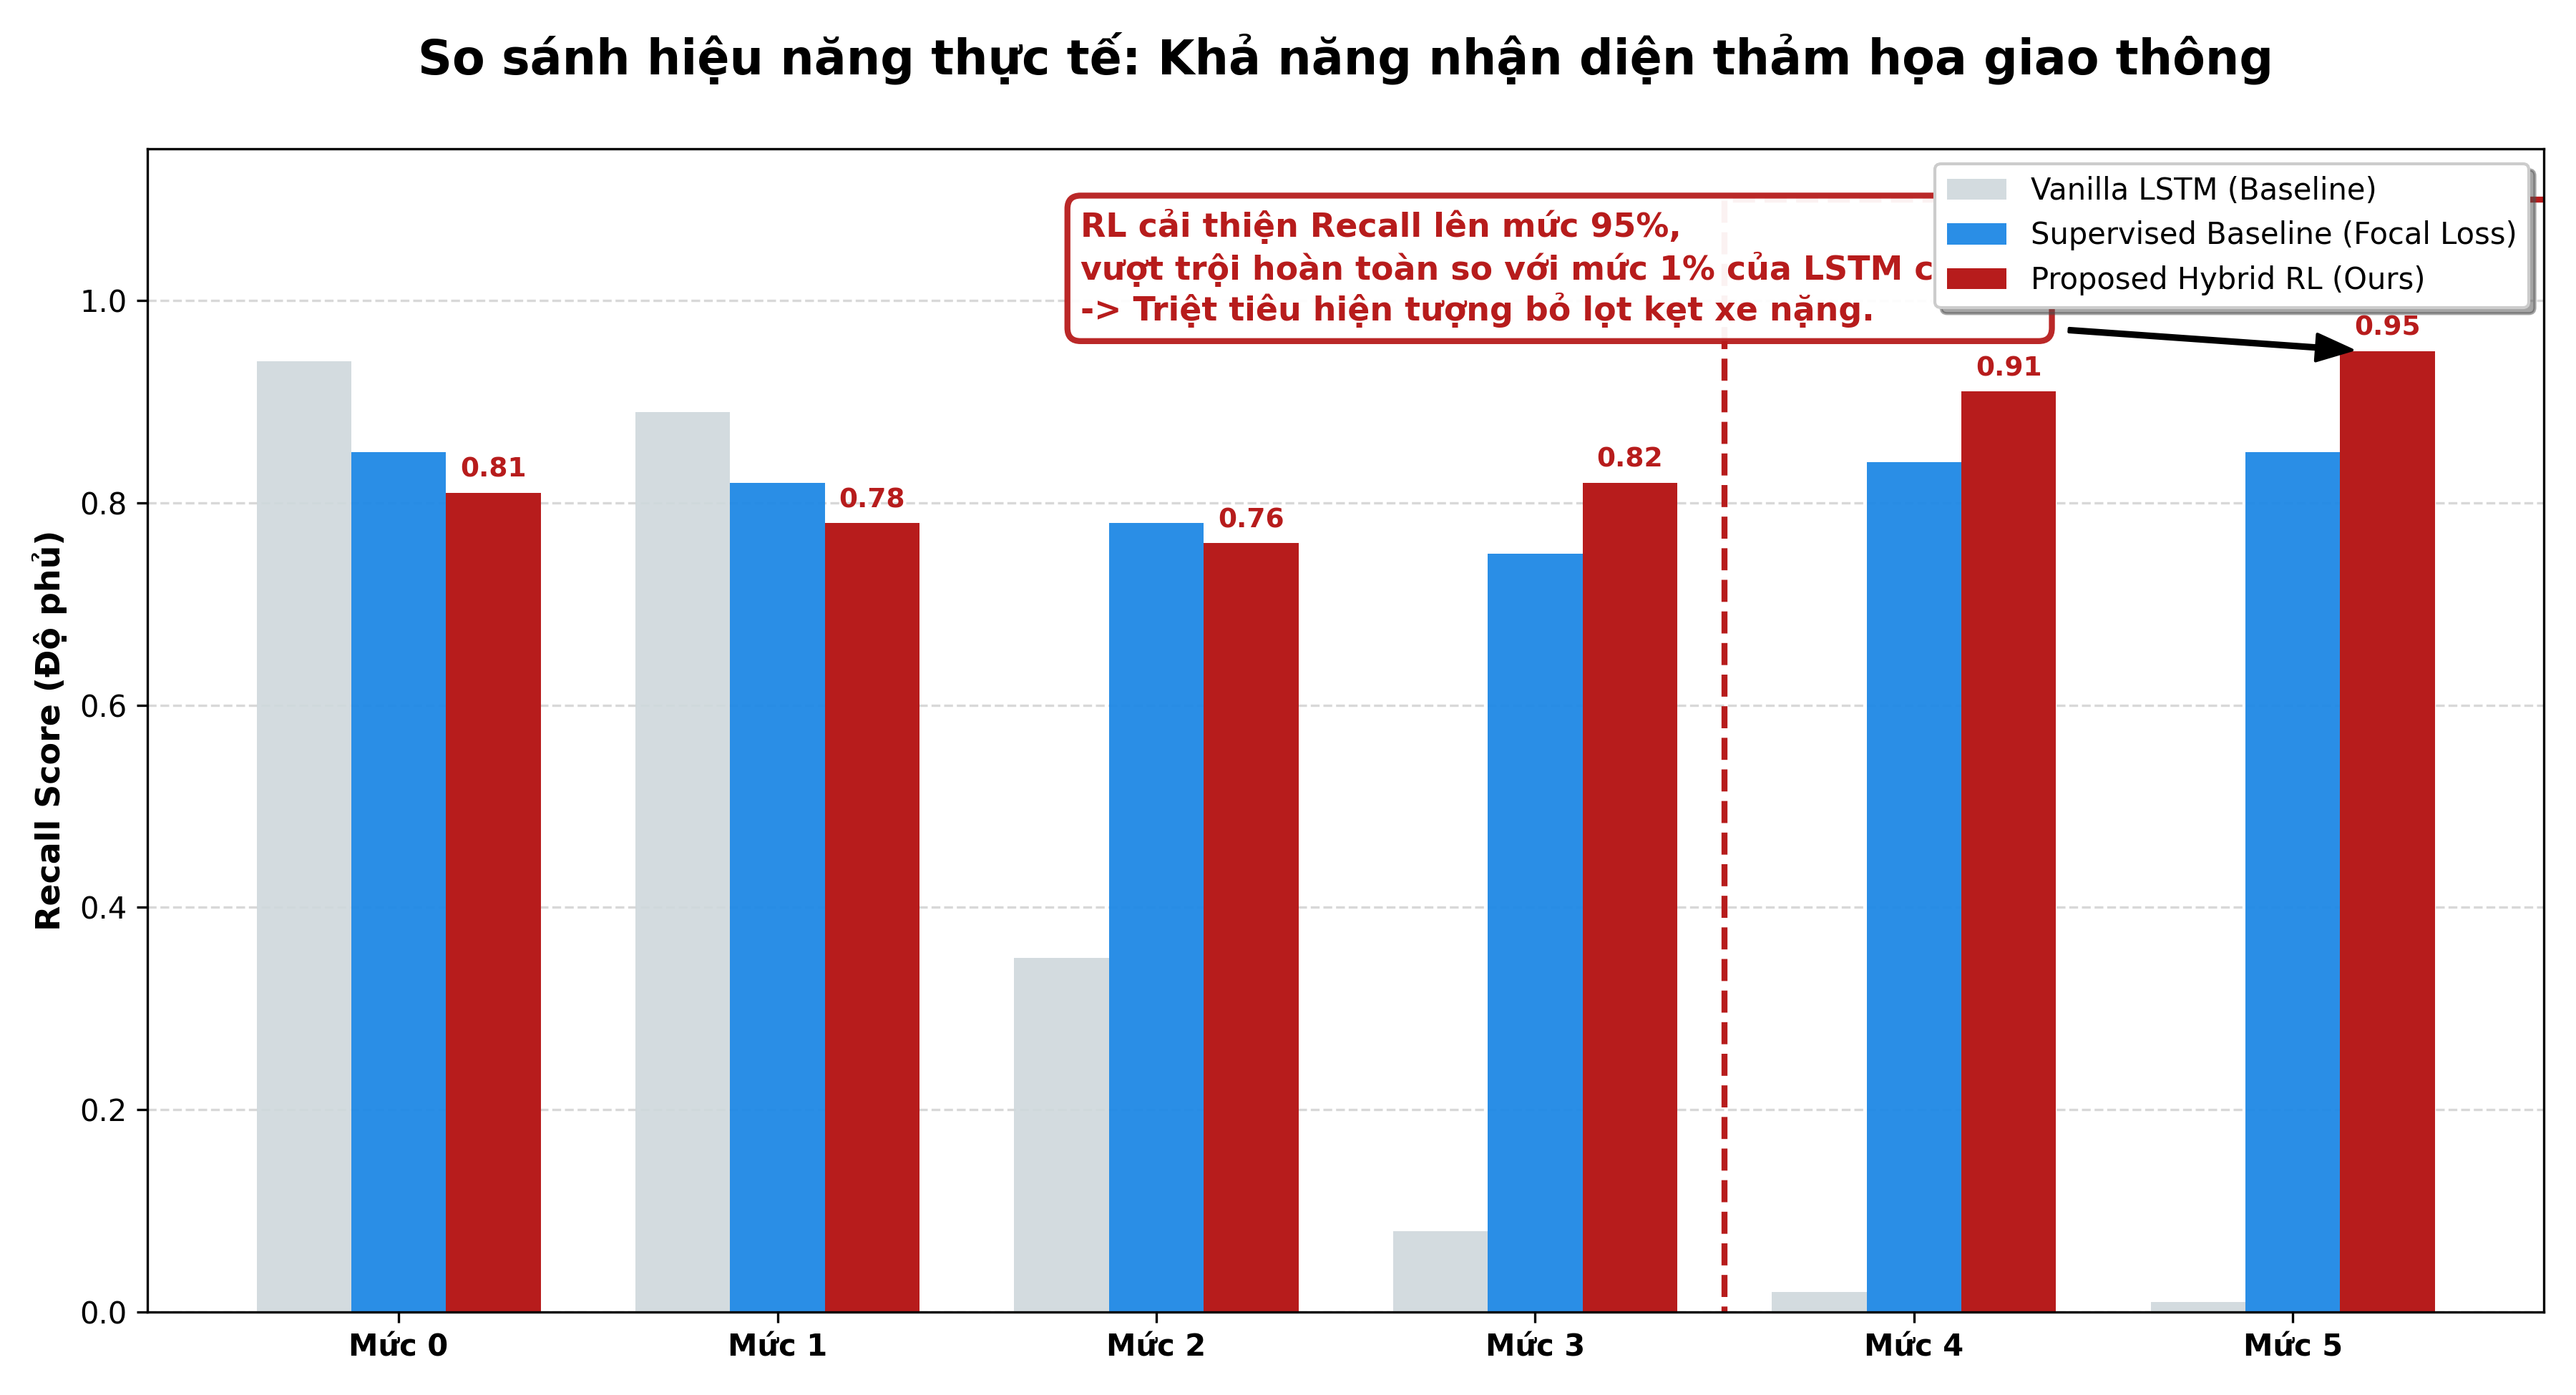
\includegraphics[width=0.8\textwidth]{Images/CH5/20.png}
    \vspace{12pt}
    \caption{Biểu đồ so sánh hiệu năng thực tế giữa các mô hình}
    \label{fig:5_20}
\end{figure}

\subsubsection{Giải mã "Hộp đen" và Tính minh bạch của hệ thống (Explainable AI với SHAP)}

\paragraph{a. Vấn đề "Hộp đen" trong Học sâu (The Black-box Problem)} \mbox{} \\
Mặc dù kiến trúc Hybrid Double DQN mang lại hiệu suất vượt trội, nó vẫn không thoát khỏi bài toán kinh điển của Học sâu: Tính minh bạch bị che khuất. Nếu không thể cung cấp lời giải thích logic mang tính vật lý, hệ thống sẽ vấp phải sự hoài nghi của người quản trị do nghi ngờ mô hình chỉ đang "học vẹt".

\paragraph{b. Giải pháp SHAP (SHapley Additive exPlanations)} \mbox{} \\
Để phá vỡ hộp đen, đồ án tích hợp lớp công nghệ \textbf{Trí tuệ nhân tạo có thể diễn giải (Explainable AI - XAI)}, sử dụng phương pháp SHAP. Thuật toán này tính toán giá trị Shapley để phân bổ công bằng tầm ảnh hưởng biên của từng đặc trưng đầu vào (vận tốc, độ trễ, thời gian) đối với kết quả dự báo cuối cùng.

\paragraph{c. Minh chứng thực tiễn: Cấu trúc logic của một cảnh báo thảm họa} \mbox{} \\
Bằng cách áp dụng SHAP để bóc tách một ca cảnh báo Thảm họa (Lớp 5), hệ thống đã trích xuất được sự đóng góp cục bộ của các biến số:
\begin{enumerate}
    \item \textbf{Dẫn dắt bởi quy luật vật lý:} Tín hiệu đẩy dự báo lên Lớp 5 mạnh mẽ nhất đến từ việc biến số \texttt{current\_speed\_kmh} giảm sâu bất thường, kết hợp với sự tăng vọt cục bộ của \texttt{traffic\_index}.
    \item \textbf{Sự tương tác phi tuyến:} SHAP phát hiện rằng giá trị SHAP của lớp 5 chỉ thực sự bùng nổ khi "Vận tốc giảm" xảy ra đồng thời với biến bối cảnh \texttt{is\_rush\_hour = True} hoặc thời tiết xấu.
    \item \textbf{Khử bỏ học vẹt:} Các biến định danh tĩnh (như \texttt{segment\_id}) có giá trị SHAP đóng góp xoay quanh mức $0$. Điều này chứng minh Đặc vụ DQN đã thực sự học được \textbf{Động lực học dòng chảy giao thông} dựa trên các nguyên lý vật lý nhân quả, thay vì chỉ cố gắng ghi nhớ thuộc tính của từng đoạn đường cụ thể.
\end{enumerate}

Sự minh bạch hóa này biến kiến trúc "Hộp đen" thành một "Hộp kính" (Glass-box), đảm bảo mọi quyết định điều hướng và cảnh báo của hệ thống đều có thể được truy vết, kiểm toán và giải thích một cách thuyết phục cho con người.
